\section{Simulation of radiation environments}
\label{sec:simulation}

{\it Editors: I.~Dawson, S.~Mallows}  \\
{\it Contibuting authors: I.~Azhgirey, I.~Dawson, M.~Huhtinen, V.~Ivantchenko, D.~Kar, M.~Karacson, S.~Mallows, I.~Mandic, A.~Di\,Mauro, S.~Menke, P.S.~Miyagawa, A.~Mucha, S.~Pospisil, T.~Szumlak, V.~Vlachoudis}  

\subsection{Introduction}
Simulating radiation environments  is crucial in the design phase of new hadron collider experiments or upgrades. 
This is especially true when extrapolating to new centre of mass collision energies where previous experience cannot be relied on. 
The generation of radiation fields in the LHC experiments is dominated by proton-proton collisions, with contributions from beam-gas interactions and other machine losses \cite{beam_bg}. 
It is therefore essential to first simulate the proton-proton collisions, using Monte Carlo event generators such as PYTHIA-8 \cite{PYTHIA} and DPMJET-III  \cite{DPMJET}. This part of the simulation is discussed in Section\,\ref{ev-gen}. 

The particles originating from the proton-proton collisions interact with the detector and machine material, causing electromagnetic and hadronic showers which give rise to the complex radiation fields seen in the LHC experiments. This second part of the simulation is dealt with using advanced Monte Carlo particle transport codes such as FLUKA  \cite{FLUKA}, MARS  \cite{MARS} or GEANT4  \cite{GEANT4}. An overview of these codes is given in Section\,\ref{sim-codes}, and their implementation in each experiment is presented in Section\,\ref{sim-frameworks}

While the simulation codes provide information on particle type, flux and energy, the detector systems want radiation quantities they can use to model and predict radiation damage effects. Examples of derived quantities include: 1 MeV neutron equivalent fluence; ionising dose; hadron flux greater than 20 MeV; radionuclide production.  This is discussed in Section\,\ref{sim-fluences}, along with summaries of the radiation background predictions from each of the experiments, 

Finally, in Section\,\ref{sim-SFs}., we explore the important topic of simulation uncertainties, which is achieved by comparing the simulated predictions with measurements.

\subsection{Event generation}
\label{ev-gen}
The physics processes in inelastic proton-proton collisions are dominated by soft (low-$p_{T}$) QCD interactions, but hard (high-$p_{T}$) parton-parton scatters can play an important role too in radiation background studies.
Experimental physicists often refer to these events as "minimum-bias", reflecting the minimally biassed trigger system required to study these events. 
Although the hard scattering processes are well described by perturbative QCD, this breaks down for low-$p_{T}$ interactions and a wide variety of models with distinct theoretical concepts have been developed to describe this regime. 

A good minimum-bias event generator describes accurately both the soft and hard physics processes, including diffractive disassociation of one or both protons.
The cross sections for these processes should be provided too so that event rates can be calculated. 
Another desirable feature is a smooth transition between the soft and hard processes up to the highest centre of mass collision energies. 
PHOJET \cite{PHOJET} (part of the DPMJET-III package) was used extensively during the design phase of the ATLAS experiment, and implements the Dual Parton Model \cite{DPM} to describe particle production in low-$p_{T}$ processes. 
PYTHIA6 \cite{PYTHIA6} was also used in the original design studies on ATLAS to provide an estimate of systematic uncertainties in the event generator predictions. An example of such a study is given in \cite{Pyth6PhojetComp}. PYTHIA6 implements leading order QCD matrix elements with very low transverse momentum cut-off to model the low-$p_{T}$ (non-diffractive) physics, and incorporates different approaches for dealing with the resulting divergences. Other well known Monte Carlo event generators at the time such as ISAJET and HERWIG had not been fully developed for minimum-bias event generation.

Since data taking started at the LHC experiments in 2009, comparisons with the Monte Carlo predictions have been made. 
Measurements of event distributions such as $dN_{ch}/d\eta$ and $dN_{ch}/d p_{T}$ have been made for centre-of-mass energies 900\,GeV, 7\,TeV and 13\,Tev, allowing tuning of the MC phenomenological models \cite{minbiasPapers}
Corresponding measurements of the proton-proton cross sections have been made, allowing the rise of the inelastic cross sections to be studied \cite{ppCrossSection}, See also Table~\ref{tab:ppXS} 

The ATLAS experiment use mainly PYTHIA8 for minimum bias event generation. This is because the code is fully supported by the LHC experiments and the code authors, with continuous development and improvement of the physics models. DPMJET-III is integrated into the FLUKA transport code and used by CMS and LHCb.


\begin{table}[h]
\begin{center}
\caption{Comparison of measured inelastic proton-proton cross sections (mb) with simulated predictions from PYTHIA8 and DPMJET-III.}
\label{tab:ppXS}
\begin{tabular}{lccccc}
\hline\hline
 & \multicolumn{3}{c}{\textbf{LHC measurements}} & \multicolumn{2}{c}{\textbf{Event generator predictions}}\\
  & \textbf{ATLAS}  & \textbf{CMS} & \textbf{LHCb} & \textbf{PYTHIA8 A3} & \textbf{DPMJET-III} \\
\hline
$\sqrt{s} =  $13\,TeV    & 68.1 $\pm$  1.4    &   &  & 69.9  & \\
$\sqrt{s} =  $7\,TeV   & 60.3  $\pm$  2.1   &     &  & 62.3 & \\
\hline\hline
\end{tabular}
\end{center}
\end{table}

\begin{figure}[ht]
\begin{center}
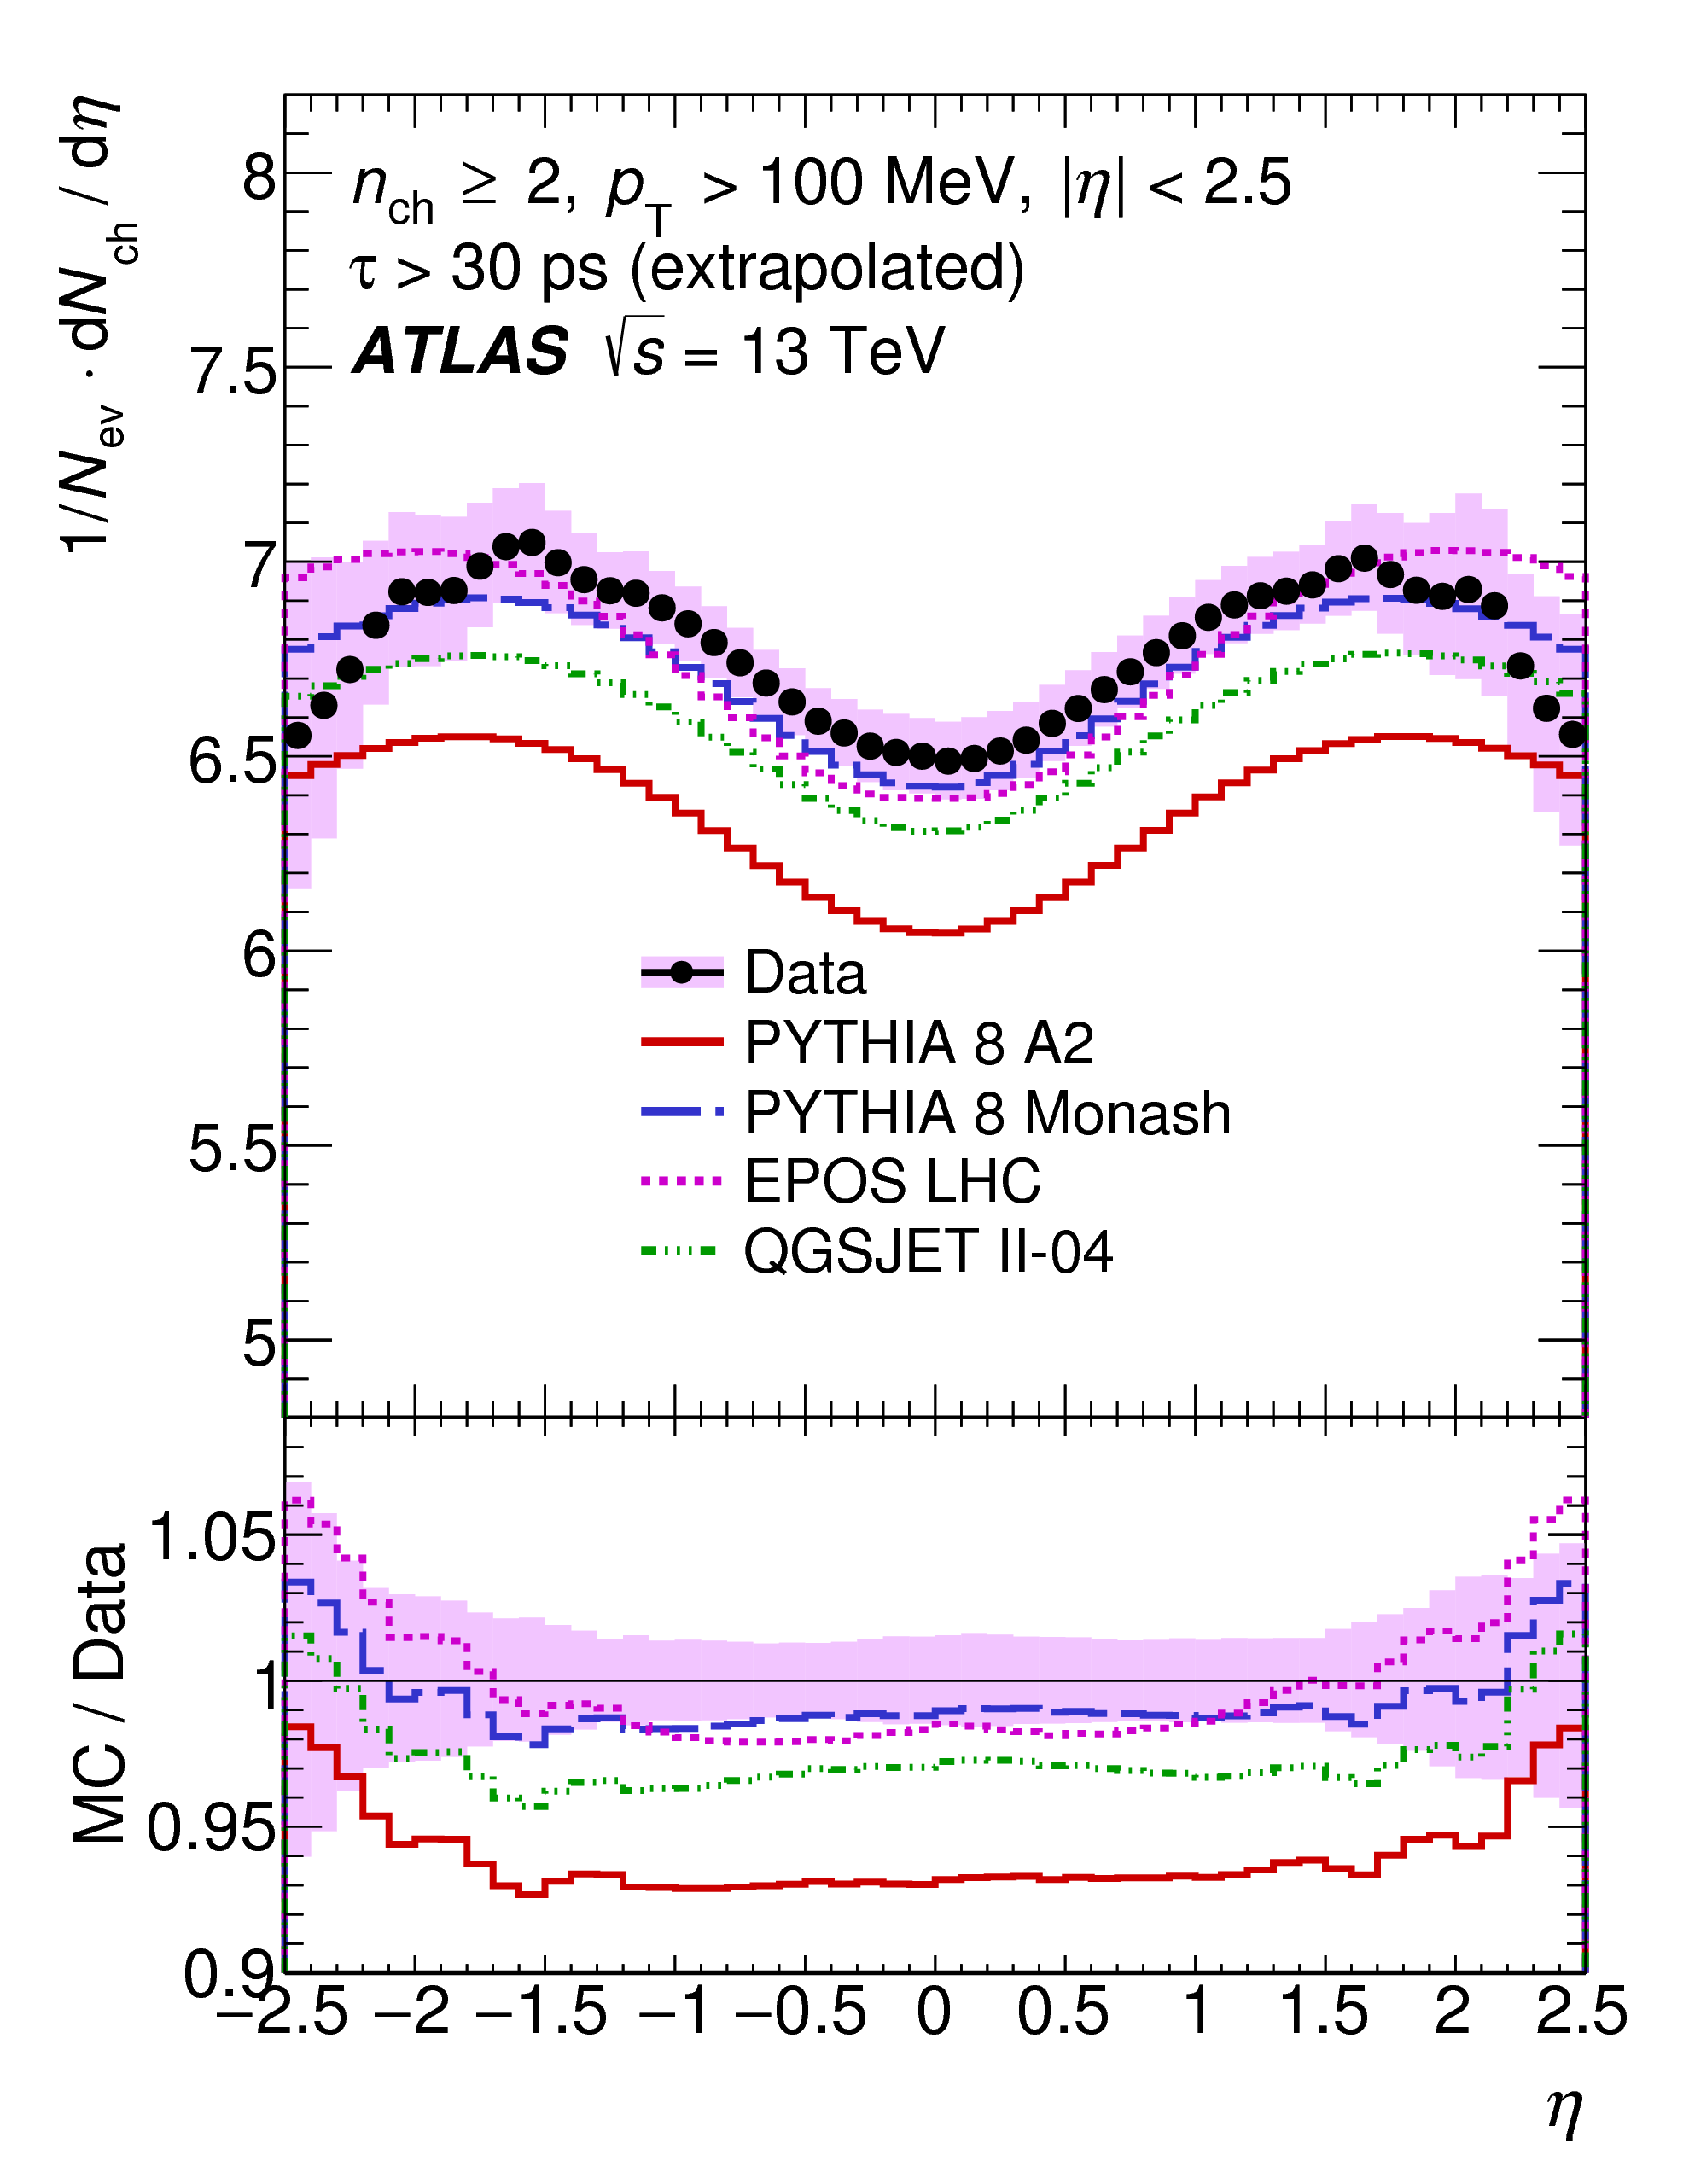
\includegraphics[width=8cm]{figures/RadiationSimulation/minbiasExample.png}
\caption{Example of ATLAS minbias plot. Is there something similar summarising the LHC experiments?}
\label{fig:line}
\end{center}
\end{figure}



\subsection{Particle transport codes}
\label{sim-codes}

General discussion on on particle transport codes used in the LHC experiments. 
At TeV hadron colliders such as the LHC, particle interactions have to be accurately modelled over a broad range of energies (typically TeV down to keV, or thermal for neutrons), for both hadronic and electromagnetic processes. 

Monte Carlo particle transport codes are essential in simulating and studying the radiation fields. 
ATLAS uses both FLUKA and GEANT4, CMS relies on FLUKA and MARS. LHCb predominantly uses FLUKA.
FLUKA has been developed at CERN over the past 40+ years and its use is widespread.



\subsubsection{FLUKA/FLUGG}
\subsubsection{MARS}
\subsubsection{GEANT4}
Give brief overview of GEANT4 physics capabilities, and how the G4 packages are maturing nicely for radiation background simulations. Advantage of using software that the rest of experiment uses for physics studies. Running on the Grid.
\subsubsection{GEANT3/CALOR}
Give brief overview of past GEANT3/CALOR studies on ATLAS, especially during initial design phase. Now superseded by GEANT4. 
However, good to make point that radiation background expertise tends to be limited, so sometimes better to be agnostic when it comes to choosing simulation strategies.


\subsection{Simulation frameworks}
\label{sim-frameworks}
For example, ATLAS uses Git repository for shared geometry development, which includes CERN Radiation Protection so they can perform radiological studies. 
Simulation results are shared with experiment groups through Web tools and TWikis pages.


\subsection{Fluence and dose predictions}
\label{sim-fluences}

\subsubsection{ATLAS}

\subsubsection{CMS}

\subsubsection{LHCb}

\subsubsection{ALICE}

\subsection{A discussion on simulation uncertainties}
\label{sim-SFs}

\begin{thebibliography}{99}

\bibitem{beam_bg} 
ATLAS Collaboration.
\textit{Comparison between simulated and observed LHC beam backgrounds in the ATLAS experiment at $E_{beam}$ = 4\,TeV}.
Journal of Instrumentation, Vol 13, Dec 2018.

\bibitem{PYTHIA} 
PYTHIA8 ref.

\bibitem{DPMJET} 
DPMJET ref.

\bibitem{FLUKA} 
FLUKA ref.
\bibitem{MARS} 
MARS ref.
\bibitem{GEANT4} 
GEANT4 ref.
\bibitem{PHOJET} 
PHOJET ref.
\bibitem{DPM} 
DPM ref.
\bibitem{PYTHIA6} 
PYTHIA6 ref.

\bibitem{Pyth6PhojetComp} 
Reference of early study comparing event generators used for LHC studies. For example:\\
ATLAS Collaboration.
\textit{Charged-particle multiplicities in pp interactions measured with the ATLAS detector at the LHC}.
 New Journal of Physics, Volume 13, May 2011

\bibitem{minbiasPapers} 
References to minbias studies and comparison to summarising pp inelastic cross section studies.

\bibitem{ppCrossSection} 
Reference summarising pp inelastic cross section studies.



\end{thebibliography}

 
